\documentclass[10pt]{article}
\usepackage{geometry}                % See geometry.pdf to learn the layout options. There are lots.
\usepackage{blindtext}
\usepackage[parfill]{parskip}    % Activate to begin paragraphs with an empty line rather than an indent
\usepackage{tikz}
\usetikzlibrary{arrows,automata,shadows,positioning,shapes}
\usepackage{graphicx}
\usepackage{amssymb}
\usepackage{amsmath}
\usepackage{amsthm}
\usepackage{epstopdf}
\usepackage{hyperref}
\usepackage{listings}
\usepackage{subfiles}
\usepackage[utf8]{inputenc}
\usepackage{float}
\usepackage{tikz}
\usepackage{graphicx}
\usepackage{caption}
\usepackage{wrapfig}

\begin{document}

\section*{Exercise 40}
  \subsection*{a)}
    \begin{displaymath}
      \varphi_a=\textbf{F}\textbf{G}( (\neg p_1 \land \neg p_2) \lor (p_1 \land \neg p_2) )
    \end{displaymath}
  \subsection*{b)}
    \begin{displaymath}
      \begin{array}{ r c l }
      \varphi_b&=&
              \textbf{F}
              \textbf{G}(\textbf{F}(\neg p_1 \land p_2) 
                  \land \textbf{F}( p_1 \land \neg p_2)
                  \land \neg \textbf{F}( p_1 \land p_2) ) 
      \end{array}
    \end{displaymath}

\section*{Exercise 41}
  \subsection*{a)}
    \begin{figure}[h]
      \centering
      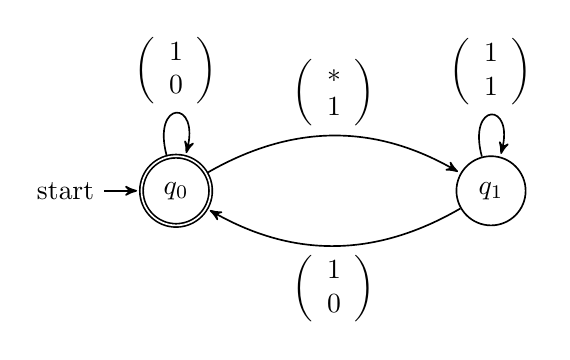
\begin{tikzpicture}[->,>=stealth',shorten >=1pt,auto,node distance=4cm,
                              semithick]

        \node[state,initial,accepting] (q0) {$q_{0}$};
        \node[state] (q1) [right of=q0] {$q_{1}$};

        \path (q0)  edge[->,bend left] node 
                  {$\left(\begin{array}{c} * \\ 1\end{array}\right)$} (q1)
                    edge[->, loop above] node
                  {$\left(\begin{array}{c} 1 \\ 0\end{array}\right)$} (q0)
              (q1)  edge[->,loop above] node 
                  {$\left(\begin{array}{c} 1 \\ 1\end{array}\right)$} (q1)
                    edge[->, bend left] node
                  {$\left(\begin{array}{c} 1 \\ 0 \end{array}\right)$} (q0);
      \end{tikzpicture}
    \end{figure}
  \subsection*{b)}
    \begin{figure}[h]
      \centering
      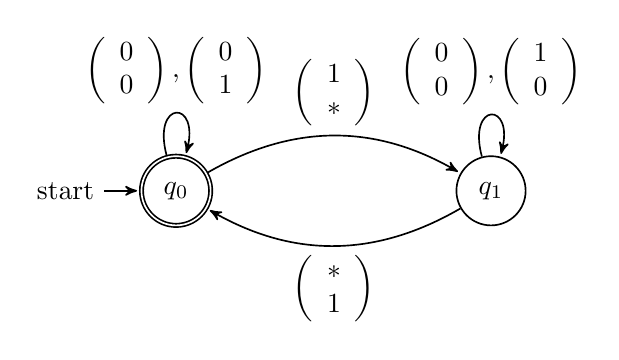
\begin{tikzpicture}[->,>=stealth',shorten >=1pt,auto,node distance=4cm,
                              semithick]

        \node[state,initial,accepting] (q0) {$q_{0}$};
        \node[state] (q1) [right of=q0] {$q_{1}$};

        \path (q0)  edge[->,bend left] node 
                      {$\left(\begin{array}{c}1\\ *\end{array}\right)$}  (q1)
                    edge[->,loop above] node
                      {$\left(\begin{array}{c}0\\0\end{array}\right),
                        \left(\begin{array}{c}0\\1\end{array}\right)$}  (q0)
              (q1)  edge[->,bend left] node
                      {$\left(\begin{array}{c}*\\1\end{array}\right)$}  (q0)
                    edge[->,loop above] node
                      {$\left(\begin{array}{c}0\\0\end{array}\right),
                        \left(\begin{array}{c}1\\0\end{array}\right)$}  (q1);
          
      \end{tikzpicture}
    \end{figure}

\section*{42}
  \subsection*{a)}
    \begin{displaymath}
      \alpha_{a}=\left( \left(\begin{array}{c}1 \\ *\end{array}\right)
                    \left(\begin{array}{c}0 \\ *\end{array}\right)
             \right)^{\omega}
    \end{displaymath}
    \begin{center}
      $\alpha_{a}\models \varphi_2$ and $\alpha_{a} \not\models \varphi_1$
    \end{center}
  \subsection*{b)}
    \begin{displaymath}
      \alpha_{b}= \left(\begin{array}{c}1\\0\\0\end{array}\right)
                  \left(\begin{array}{c}0\\1\\0\end{array}\right)
                  \left(\begin{array}{c}0\\0\\1\end{array}\right)^\omega
    \end{displaymath}
    \begin{center}
      $\alpha \models \psi_1$ and $\alpha \not\models \psi_2$
    \end{center}

\section*{43}
  \subsection*{a)}
    \begin{displaymath}
      \varphi_{a}=  p_1 \land \textbf{X}\neg p_1\land
                    \textbf{G}(\textbf{XXX}\neg p_1 
                          \land \textbf{XXXX}p_1 
                          \land \textbf{XXXXX}p_1
                          \land p_1 \rightarrow \textbf{XXX}p_1)
    \end{displaymath}
%    $\alpha \models \varphi_{a}$. The first two letters of $\alpha$ must be an
%    $10$ which is given by $p_1\land \textbf{X}\neg p_1$ so $alpha$ must have a
%    form like $\alpha=10\cdot w$. The second part of the formula
%    $\textbf{G}\varphi$

  \subsection*{b)}
    \begin{displaymath}
      \varphi_{b}=\varphi_{u}\textbf{G}\varphi_{v}
    \end{displaymath}
  
    The part $\varphi_{u}$, where $\varphi_{u}$ describes the word $u$, guaranties 
    that the word $\alpha$ has to start with $u$ and the second part 
    $\textbf{G}\varphi_{v}$, where $\varphi_{v}$ describes the word $v$
    guaranties that the word $v$ is repeated infinitely often.
    
    

\end{document}

